\documentclass[11pt]{article}

\usepackage[review]{acl}
\usepackage{times}
\usepackage{latexsym}
\usepackage{amsmath}
\usepackage{amssymb}
\usepackage{booktabs}
\usepackage{graphicx}
\usepackage{microtype}
\usepackage{url}

\title{Does Quantization Change What Agreement Means?\\
A Paired Audit of Homogeneous LLM Panels}

\author{Anonymous UncertaiNLP submission}

\newcommand{\nf}{\textsc{nf4}}
\newcommand{\fp}{\textsc{fp16}}

\begin{document}
\maketitle

\begin{abstract}
Agreement among repeated large language model (LLM) samples is often treated as confidence, but compression may change the dependence behind that agreement. We present a paired audit of homogeneous five-member panels from the same checkpoints at \fp{} and 4-bit \nf{}. We evaluate two open models on 300 TruthfulQA multiple-choice questions and 300 GSM8K problems, using matched prompts, sampling settings, and seeds. Quantization reduces panel accuracy on GSM8K by 10.5 percentage points for Qwen2.5-3B and 6.3 points for Phi-3.5-mini, while increasing the probability that all five members fail by 9.0 and 5.0 points. It also raises invalid structured answers by 12.5 and 7.5 points. Agreement becomes a worse selective-confidence signal on both models. However, conditional same-wrong-answer concentration changes little and inconsistently. On TruthfulQA, Phi degrades while Qwen is largely stable. These results suggest a narrower conclusion than ``quantization creates consensus'': under our setup, quantization changes collective reliability mainly by increasing failure incidence and format failure, not by universally concentrating panels on one wrong answer.
\end{abstract}

\section{Introduction}

Sampling a language model several times gives a simple uncertainty signal: if the answers agree, we are more willing to trust them. Self-consistency and multi-response uncertainty methods aggregate or compare several answers \citep{wang2023selfconsistency,feng-etal-2025-rethinking,kruse-etal-2025-muse}, while multi-agent debate can explicitly communicate agent confidence \citep{yoffe-etal-2025-debunc}. The signal is useful, but it assumes that agreement keeps the same meaning after the system changes.

Quantization is one such change. It makes open LLMs much cheaper to run, but recent work shows that compressed models can lose calibration even when their accuracy changes only modestly \citep{zhong-etal-2025-quantized,tong2026compression}. Existing studies mainly examine a model's marginal confidence or prediction sets. A panel depends on a joint distribution instead: five members can keep similar marginal accuracy while becoming more likely to fail together, or they can fail more often without concentrating on the same wrong answer. Those cases should not be treated as one phenomenon.

We study this distinction with a controlled, small-scale audit. For each checkpoint, task, and question, we compare five independently sampled responses at \fp{} and locally quantized \nf{}. We separate three questions: does quantization change individual and panel accuracy; does it increase the all-members-wrong tail; and, conditional on that tail, does it make members choose the same wrong answer? We also test whether maximum vote share remains useful for ranking reliable panel decisions.

Our results are mixed in a useful way. On open-response mathematics, \nf{} consistently lowers accuracy, raises co-failure, increases format invalidity, and worsens selective reliability. On multiple choice, Phi-3.5-mini degrades but Qwen2.5-3B is stable. Yet identical-wrong concentration does not move consistently. The main lesson is therefore not that quantization always creates shared mistakes. It is that agreement-based uncertainty can degrade through more than one route, and raw consensus counts blur those routes.

\section{Related Work}

\paragraph{Compression and uncertainty.}
Quantized LLMs can be worse calibrated, with soft-prompt recovery demonstrated by \citet{zhong-etal-2025-quantized}. Conformal and broader evaluations show accuracy--uncertainty decoupling and precision-sensitive changes in calibration, error ranking, and robustness \citep{tong2026compression,tao2025revisiting,ayadi2026reliability}. These studies examine single-model or marginal quantities; we target errors across repeated members of one quantized checkpoint.

\paragraph{Agreement and collective uncertainty.}
Multi-sample and multi-agent methods estimate uncertainty from response diversity or structured semantic disagreement \citep{feng-etal-2025-rethinking,kruse-etal-2025-muse,jiang2026discouq}; accuracy-adjusted correctness dependence also predicts ensemble lift \citep{ali2026diversity}. Communication-aware work further shows that interaction can create correlated failure and false consensus \citep{huang2026cagecal}. We use no communication: each panel is five independent samples from the same model. This removes topology as a cause and isolates the precision intervention. We report the all-wrong rate $\beta$, following the observation that pairwise correlation does not determine the joint failure tail \citep{chen2026cofailure}, and separately measure whether co-failing members land on the same wrong answer.

\section{Paired Panel Audit}

\subsection{Models, tasks, and generation}

We evaluate Qwen2.5-3B-Instruct \citep{qwen2024qwen25} and Phi-3.5-mini-instruct \citep{abdin2024phi3}. Each original checkpoint is loaded in \fp{} and quantized locally with bitsandbytes \nf{}, double quantization, and \fp{} computation \citep{dettmers2023qlora}. This is weight-only post-training quantization; prompts and decoding are unchanged.

We take a fixed 300-example subset from TruthfulQA MC1 \citep{lin-etal-2022-truthfulqa} and GSM8K \citep{cobbe2021gsm8k}. For each question and precision, we draw $K=5$ members with temperature 0.7, top-$p$ 0.9, and matched seeds. TruthfulQA requests one option letter with at most 8 new tokens. GSM8K requests a derivation ending in \texttt{FINAL: <number>} with at most 256 new tokens. A missing explicit marker is invalid. We count it as incorrect and as a distinct abstention in voting, so two unparseable texts never become evidence of agreement.

The panel uses plurality vote. When several answers tie, we report expected accuracy under uniform tie-breaking rather than favoring the first member. This matters for free response, where ties are common.

\subsection{Metrics}

Let $z_{ik}\in\{0,1\}$ denote whether member $k$ is correct on question $i$, and let $F_i$ denote the event that all $K$ members are wrong. Alongside mean individual and panel accuracy, we measure the group failure tail
\begin{equation}
\beta=N^{-1}\sum_{i=1}^{N}\mathbf{1}[F_i].
\end{equation}
Among co-failures, we then measure same-wrong-answer concentration
\begin{equation}
\kappa=\Pr(a_{i1}=\cdots=a_{iK}\neq y_i\mid F_i).
\end{equation}
The numerator requires five valid answers. Thus $\beta$ captures collective failure incidence, while $\kappa$ asks whether those failures collapse onto one answer.

For agreement-based confidence, $c_i$ is the largest answer count divided by $K$. We report Brier score and area under the risk--coverage curve (AURC; lower is better). AURC tests whether high-agreement panels can be retained before low-agreement panels. We average over all orderings within vote-share ties. All \nf{}--\fp{} intervals use 10,000 paired question-level bootstrap samples.

\begin{table*}[t]
\centering
\small
\setlength{\tabcolsep}{4.2pt}
\begin{tabular}{llcrrrrrrr}
\toprule
Model & Task & Prec. & Ind. & Panel & $\beta$ & Invalid & $\kappa$ & Brier & AURC \\
\midrule
Qwen2.5-3B & TruthfulQA & FP16 & 49.7 & 49.3 & 49.0 & 0.0 & 93.9 & 0.485 & 0.486 \\
Qwen2.5-3B & TruthfulQA & NF4 & 48.3 & 48.0 & 50.7 & 0.0 & 92.8 & 0.496 & 0.499 \\
Qwen2.5-3B & GSM8K & FP16 & 51.8 & 62.3 & 26.3 & 41.9 & 1.3 & 0.093 & 0.102 \\
Qwen2.5-3B & GSM8K & NF4 & 41.0 & 51.9 & 35.3 & 54.4 & 0.0 & 0.095 & 0.158 \\
\midrule
Phi-3.5-mini & TruthfulQA & FP16 & 54.9 & 55.8 & 43.0 & 0.0 & 84.5 & 0.409 & 0.415 \\
Phi-3.5-mini & TruthfulQA & NF4 & 50.2 & 50.0 & 48.0 & 0.0 & 86.8 & 0.455 & 0.466 \\
Phi-3.5-mini & GSM8K & FP16 & 33.5 & 47.5 & 39.3 & 63.3 & 0.0 & 0.113 & 0.195 \\
Phi-3.5-mini & GSM8K & NF4 & 26.5 & 41.1 & 45.0 & 70.6 & 0.7 & 0.126 & 0.264 \\
\bottomrule
\end{tabular}
\caption{Absolute results (\%). Brier and AURC are unitless; lower is better. $\beta$ is the all-members-wrong rate and $\kappa$ is same-wrong-answer concentration conditional on co-failure. Invalid outputs are treated as distinct abstentions, not agreement.}
\label{tab:absolute}
\end{table*}


\section{Results}

\begin{figure*}[t]
\centering
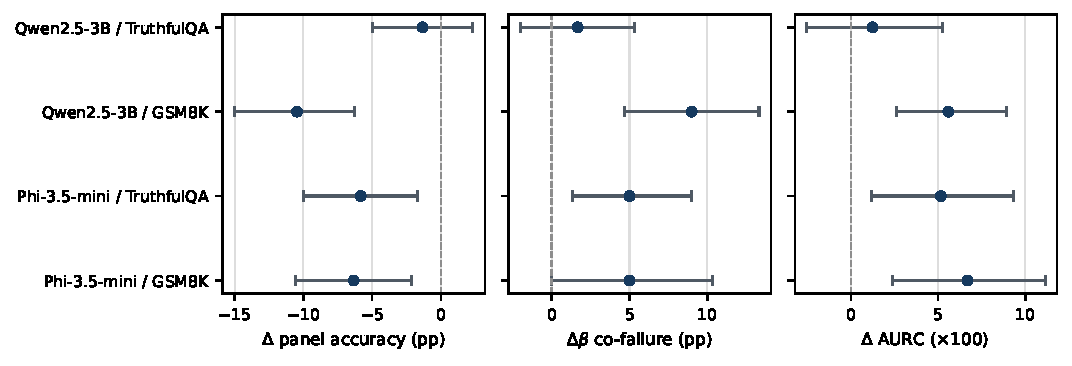
\includegraphics[width=\textwidth]{figures/delta_summary.pdf}
\caption{Paired \nf{} minus \fp{} effects with 95\% question-bootstrap intervals. Negative panel-accuracy values and positive $\beta$/AURC values indicate degradation. Quantization reliably hurts both GSM8K panels and Phi on TruthfulQA; Qwen on TruthfulQA is stable.}
\label{fig:deltas}
\end{figure*}

\subsection{Quantization raises collective failure}

Table~\ref{tab:absolute} and Figure~\ref{fig:deltas} show a consistent GSM8K pattern. For Qwen, \nf{} changes individual accuracy by $-10.8$ points (95\% CI $[-13.7,-8.0]$), panel accuracy by $-10.5$ $[-15.0,-6.3]$, and $\beta$ by $+9.0$ $[4.7,13.3]$. Phi follows the same direction: individual accuracy changes by $-6.9$ $[-9.7,-4.1]$, panel accuracy by $-6.3$ $[-10.6,-2.1]$, and $\beta$ by $+5.0$ $[0.0,10.3]$.

The multiple-choice result is model-dependent. Phi loses 4.7 points of individual accuracy and 5.8 points of panel accuracy, with $\beta$ increasing by 5.0 points. All three intervals exclude zero. Qwen changes by less than two points on the same task, and its intervals include zero. Quantization therefore has a reproducible effect on open-response reasoning in our two models, but not a universal effect across formats.

\subsection{More co-failure is not the same as more wrong consensus}

TruthfulQA naturally produces high same-wrong concentration because all members choose from a small option set. Still, \nf{} barely changes conditional concentration: Qwen moves from 93.9\% to 92.8\% ($\Delta\kappa=-1.1$, CI $[-6.3,4.1]$), while Phi moves from 84.5\% to 86.8\% ($+2.3$, $[-4.6,9.4]$). The directions disagree and both intervals cross zero. Phi's unconditional same-wrong rate does rise by 5.3 points, but this is explained mainly by the larger co-failure pool rather than a clear change in $\kappa$.

On GSM8K, exact same-wrong events are almost absent: one event for Qwen \fp{}, none for Qwen \nf{} or Phi \fp{}, and one for Phi \nf{}. This does not imply that the panels are reliable. The strict final-answer failure rate is already 41.9--63.1\% at \fp{}, and \nf{} raises it by 12.5 points for Qwen and 7.5 for Phi; both intervals exclude zero. The complete-parse subset is consequently too small for a useful free-response $\kappa$ sensitivity estimate. We report this sparsity rather than turning truncated derivations into guessed numeric answers.

\subsection{Agreement becomes a worse ranking signal}

AURC increases by 5.6 points for Qwen GSM8K and 6.7 for Phi GSM8K; both bootstrap intervals exclude zero. Phi TruthfulQA also worsens by 5.2 points, while Qwen TruthfulQA remains stable. Brier score is less sensitive: it significantly worsens only for Phi TruthfulQA ($+0.046$, CI $[0.009,0.085]$). This difference is informative. Quantization more consistently harms the ordering induced by agreement---which questions look safest---than the average squared calibration loss at a few discrete vote shares.

Taken together, the results separate two effects that a raw consensus rate would merge. \nf{} often creates more opportunities for collective failure, but we do not find consistent evidence that a co-failing panel becomes more likely to select one identical wrong answer.

\section{Limitations}

This is a controlled case study, not a universal quantization benchmark. It covers two small model families, one 4-bit method, two tasks, and 300 fixed questions per task. The members are independent samples from a homogeneous checkpoint, not role-specialized or communicating agents. Exact numeric matching is suitable for GSM8K, but the required final marker and 256-token cap produce many invalid outputs; this is partly a protocol-adherence result and partly an evaluation limitation. Multiple-choice format also anchors answers to a small set, so its high $\kappa$ should not be compared directly with free response. Finally, vote share has only a few levels, which is why we emphasize Brier, AURC, and paired intervals instead of relying on ECE.

\section{Conclusion}

Within those bounds, the result is clear. Quantization can change what panel agreement means, but the change is not a single rise in ``false consensus.'' In our setup it appears mainly as lower accuracy, a heavier all-wrong tail, more invalid structured answers, and weaker selective reliability. Keeping failure incidence separate from failure concentration gives a simpler and more honest audit of compressed LLM panels.

\bibliography{references}

\appendix
\clearpage

\section{Sensitivity Analysis}

\paragraph{Chance-adjusted concentration.}
For TruthfulQA, we also subtract a stratified independence baseline that preserves each member's wrong-answer frequencies within the gold-label stratum. The \nf{}--\fp{} change in excess $\kappa$ is $+1.2$ points for Qwen (95\% CI $[-4.6,7.3]$) and $+2.9$ for Phi ($[-4.4,10.6]$). These intervals agree with the raw $\kappa$ analysis: the finite answer set creates substantial wrong agreement, but its excess concentration does not change reliably under \nf{}.

\section{Reproducibility Details}

The experiment uses five samples per question and base seed 20260809, with member seed $20260809+5i+k$. The final runtime uses Transformers 4.57.6, bitsandbytes 0.50.0, and \fp{} compute for \nf{}. Phi remote model code is pinned to revision \texttt{2fe1924}. Raw JSONL generations, configuration files, environment records, analysis code, and 10,000-replicate bootstrap outputs are included in the anonymous supplementary material.

\section{Prompt Templates}

TruthfulQA uses: \emph{``Answer the multiple-choice question by returning only the single option letter. Do not explain your answer.''} GSM8K uses: \emph{``Solve the problem step by step. End with exactly FINAL: <number>. The final marker is required.''} No demonstrations or communication between members are used.

\end{document}
